
%(BEGIN_QUESTION)
% Copyright 2008, Tony R. Kuphaldt, released under the Creative Commons Attribution License (v 1.0)
% This means you may do almost anything with this work of mine, so long as you give me proper credit

Three-phase electric motors are often equipped with a set of electrical terminals for configuring different voltage ranges and/or base speeds.  Different configurations consist of different patterns of ``jumper'' wires connecting these terminals together.  For example, here is an illustration of a three-phase electric motor with nine stud-and-nut terminals for connecting a set of six wire windings (coils) in two different configurations: one for low voltage (240 volts AC) and one for high voltage (480 volts AC):

$$\includegraphics[width=15.5cm]{i02298x01.eps}$$

When connecting the terminals for high-voltage operation, the goal is to have a ``delta'' configuration with two series-connected windings in each side of the triangle.  When connecting the terminals for low-voltage operation, the goal is to have two parallel ``delta'' winding sets.

\vskip 10pt

Sketch the proper power conductor and jumper connections for low-voltage operation and for high-voltage operation:

$$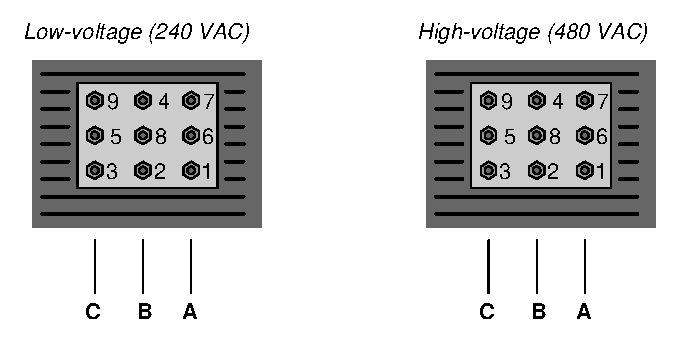
\includegraphics[width=15.5cm]{i02298x03.eps}$$

\vskip 20pt \vbox{\hrule \hbox{\strut \vrule{} {\bf Suggestions for Socratic discussion} \vrule} \hrule}

\begin{itemize}
\item{} Why do you think an electric motor manufacturer would equip one of their motors with the capability of dual-voltage operation?
\end{itemize}

\underbar{file i02298}
%(END_QUESTION)





%(BEGIN_ANSWER)

This is just an exercise in connecting the dots!  A helpful problem-solving technique to apply to such problems is {\it tracing all connections made} in the schematic diagram after making those connections in the pictorial diagram.  This helps you keep track of which connections have been made, and which connections still need to be made.

$$\includegraphics[width=15.5cm]{i02298x02.eps}$$

$$\includegraphics[width=15.5cm]{i02298x04.eps}$$
 
%(END_ANSWER)





%(BEGIN_NOTES)


%INDEX% Pictorial circuit review (3-phase motor connections)

%(END_NOTES)


